% sips -s format png your_pdf_file.pdf --out your_png_file.png

\documentclass[tikz,border=0mm]{standalone}

\usepackage{amsmath}
\usepackage{graphicx}
\usepackage[T1]{fontenc}
\renewcommand\familydefault{\sfdefault} 

\usetikzlibrary{arrows,shapes,calc,math,decorations.fractals,patterns,backgrounds,decorations.markings,decorations.pathmorphing,decorations.pathreplacing,fit}

\definecolor{mygreen}{rgb}{0,0.5,0}
\tikzset{point/.style={fill,circle,inner sep=1.5pt}}
\tikzset{vector/.style={-triangle 45, line width=1pt}}
\tikzset{dblarrow/.style={latex'-latex'}}
\tikzset{partial ellipse/.style args={#1:#2:#3}{insert path={+ (#1:#3) arc (#1:#2:#3)}}}
\tikzset{axis/.style={-stealth',line width=1pt}}
\renewcommand{\vec}{\mathbf}

\tikzstyle{every picture}+=[font=\sffamily]

\makeatletter
\newcommand{\gettikzxy}[3]{%
    \path #1;%
    \edef#2{ \strip@pt\pgf@x }%
    \edef#3{ \strip@pt\pgf@y }%
}
\makeatother

% Command to draw one textured triangle
% #1-#3 are coordinates of the triangle
% #4-#6 are texture coordinates in [0,1]^2 of the image
%       where (0,0) is bottom left
% #7 is the name of the image
\newcommand\texturedtriangle[7]{%
    % Decode all the coordinates into nice single numbers
    \gettikzxy{#1}{\ax}{\ay}
    \gettikzxy{#2}{\bx}{\by}
    \gettikzxy{#3}{\cx}{\cy}
    \gettikzxy{#4}{\tax}{\tay}
    \gettikzxy{#5}{\tbx}{\tby}
    \gettikzxy{#6}{\tcx}{\tcy}
    \gettikzxy{(1,1)}{\ux}{\uy}
    % Compute the required affine transformation
    \pgfmathsetmacro\det{\tax*(\tcy-\tby) + \tay*(\tbx-\tcx) - \tbx*\tcy + \tby*\tcx}
    \pgfmathsetmacro\aa{(\ax*(\tcy-\tby) + \tay*(\bx-\cx) - \bx*\tcy + \tby*\cx)/\det}
    \pgfmathsetmacro\ba{(\ax*(\tbx-\tcx) + \tax*(\cx-\bx) - \tbx*\cx + \bx*\tcx)/\det}
    \pgfmathsetmacro\ab{(\ay*(\tcy-\tby) + \tay*(\by-\cy) - \by*\tcy + \tby*\cy)/\det}
    \pgfmathsetmacro\bb{(\ay*(\tbx-\tcx) + \tax*(\cy-\by) - \tbx*\cy + \by*\tcx)/\det}
    \pgfmathsetmacro\tx{\ax - (\tax*\aa + \tay*\ba)}
    \pgfmathsetmacro\ty{\ay - (\tax*\ab + \tay*\bb)}
    \pgflowlevelobj{
        \pgfsettransformentries{\aa}{\ab}{\ba}{\bb}{\tx pt}{\ty pt}
    }{
        % We are inside the texture space here...
        \clip #4 -- #5 -- #6 -- cycle;
        % Draw a unit sized image (from (0,0) to (1,1) if no scale)
        \node [opacity=0.5] at (0.5,0.5) {\includegraphics[width=\ux pt, height=\uy pt]{#7}};
    }
}

% Command to draw one textured triangle (lighter)
\newcommand\texturedtrianglelight[7]{%
    % Decode all the coordinates into nice single numbers
    \gettikzxy{#1}{\ax}{\ay}
    \gettikzxy{#2}{\bx}{\by}
    \gettikzxy{#3}{\cx}{\cy}
    \gettikzxy{#4}{\tax}{\tay}
    \gettikzxy{#5}{\tbx}{\tby}
    \gettikzxy{#6}{\tcx}{\tcy}
    \gettikzxy{(1,1)}{\ux}{\uy}
    % Compute the required affine transformation
    \pgfmathsetmacro\det{\tax*(\tcy-\tby) + \tay*(\tbx-\tcx) - \tbx*\tcy + \tby*\tcx}
    \pgfmathsetmacro\aa{(\ax*(\tcy-\tby) + \tay*(\bx-\cx) - \bx*\tcy + \tby*\cx)/\det}
    \pgfmathsetmacro\ba{(\ax*(\tbx-\tcx) + \tax*(\cx-\bx) - \tbx*\cx + \bx*\tcx)/\det}
    \pgfmathsetmacro\ab{(\ay*(\tcy-\tby) + \tay*(\by-\cy) - \by*\tcy + \tby*\cy)/\det}
    \pgfmathsetmacro\bb{(\ay*(\tbx-\tcx) + \tax*(\cy-\by) - \tbx*\cy + \by*\tcx)/\det}
    \pgfmathsetmacro\tx{\ax - (\tax*\aa + \tay*\ba)}
    \pgfmathsetmacro\ty{\ay - (\tax*\ab + \tay*\bb)}
    \pgflowlevelobj{
        \pgfsettransformentries{\aa}{\ab}{\ba}{\bb}{\tx pt}{\ty pt}
    }{
        % We are inside the texture space here...
        \clip #4 -- #5 -- #6 -- cycle;
        % Draw a unit sized image (from (0,0) to (1,1) if no scale)
        \node [opacity=0.5] at (0.5,0.5) {\includegraphics[width=\ux pt, height=\uy pt]{#7}};
    }
}

\begin{document}

% Graphics hardware
\begin{tikzpicture}[background rectangle/.style={fill=white}, show background rectangle,node distance=2cm]
    \node (keyboard) {\includegraphics[width=2cm]{keyboard_and_mouse.jpeg}};
    \node [draw,fill=blue!10,line width=1,rounded corners, right of=keyboard,text width=2cm,align=center,minimum height=0.75cm,node distance=3cm] (cpu) {CPU};
    \node [draw,fill=yellow!10,line width=1,rounded corners,below of=cpu,text width=2cm,align=center,minimum height=0.75cm] (memory) {Memory};
    \node [draw,fill=blue!10,line width=1,rounded corners, right of=cpu,minimum width=2cm,minimum height=0.75cm,node distance=3.5cm] (gpu) {GPU};
    \node [draw,fill=yellow!10,line width=1,rounded corners, below of=gpu,minimum width=2cm,minimum height=0.75cm,text width=2cm,align=center,xshift=-0.5cm,yshift=-0.6cm] (frame buffer) {Frame buffer};
    \node [draw,fill=yellow!10,line width=1,rounded corners, below of=gpu,minimum width=2cm,minimum height=0.75cm,text width=2cm,align=center] (graphics memory) {Graphics memory};
    \node [right of=graphics memory,node distance=3cm] (display) {\includegraphics[width=2cm]{display.png}};
    \node (box) [draw=red,line width=1,dashed,rounded corners,fit = (gpu) (graphics memory) (frame buffer)] {};
    \node [above of=box,node distance=2.2cm] {Graphics subsystem};
    \draw [<->,line width=1,shorten >= 2pt,shorten <= 2pt] (cpu) -- (memory);
    \draw [->,line width=1,shorten >= 2pt,shorten <= 2pt] (keyboard) -- (cpu);
    \draw [->,line width=1,shorten >= 2pt,shorten <= 2pt] (cpu) -- (gpu);
    \draw [<->,line width=1,shorten >= 2pt,shorten <= 2pt] (gpu) -- (graphics memory);
    \draw [->,line width=1,shorten >= 2pt,shorten <= 2pt] (graphics memory) -- (display);
\end{tikzpicture}

% C++ diagram
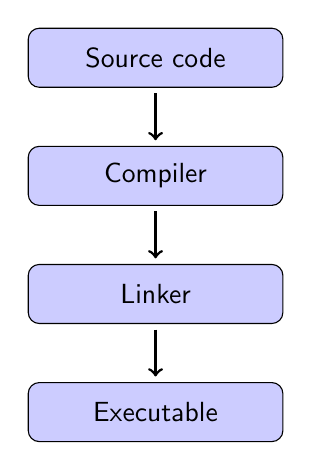
\begin{tikzpicture}[every node/.style={draw,fill=blue!20,rounded corners,text width=3cm,align=center,minimum height=0.75cm},
    node distance=1.5cm]
    \node (source) {Source code};   
    \node (compiler) [below of=source] {Compiler};
    \node (linker) [below of=compiler] {Linker};
    \node (executable) [below of=linker] {Executable}; 
    \path [->,line width=1,shorten >= 2pt,shorten <= 2pt] (source) edge (compiler) (compiler) edge (linker) (linker) edge (executable);
\end{tikzpicture}

\end{document}